% Preamble
\documentclass[12pt, a4paper]{article}
\title{\emph{Best Books for Human\\Emotions} \& \emph{Disorders}}
\author{Written by Volunteers}
\date{July 12, 2021}

% Packages
\usepackage{sectsty}
\usepackage{xcolor}
\usepackage{caption}
\usepackage[utf8]{inputenc}
\usepackage{hyperref}
\usepackage{graphicx}
\graphicspath{{images/}}

% Settings
\setcounter{tocdepth}{2}
\sectionfont{\itshape}%
\subsectionfont{\itshape}%
\subsubsectionfont{\itshape}%

% Macros
\newcommand{\nl}{\vspace{\baselineskip}}
\newenvironment{additional}{%
    \begin{list}{}%
        {\setlength{\leftmargin}{\parindent}}%
        \item[]%
        Additional:
        \begin{itemize}}
    {\end{itemize}\end{list}}

% Body
\begin{document}
\maketitle

\section*{Categories and contribution}
Despite the fact that the list is still a work in progress, one could add to
categories or introduce books to the ones listed here. At the moment, table of
content only includes categories with more than one entry.
\begin{enumerate}
    \item Social Skills
    \item Generalized Anxiety Disorder
    \item Social Anxiety Disorder \& Shyness
    \item Overthinking
    \item Jealousy
    \item Self-awareness
    \item Self-consciousness
    \item Happiness
    \item Paranoia
    \item Revenge
    \item Self-confidence / Self-esteem
    \item False Self-confidence / Self-esteem
    \item Addiction
    \item OCD
    \item Perfectionism
    \item Child Abuse
    \item Painful Past
    \item Panic Attack
    \item Self-harm / Self-injury
    \item Suicide
    \item Trauma
    \item Post Traumatic Stress Disorder
    \item Shizoaffective
    \item Shizophernia
    \item Hallucinations
    \item Delusional Disorder
    \item Major Depressive Disorder
    \item Dysthymia
    \item Bipolar Disorder
\end{enumerate}

\begin{figure}[hb]\centering
    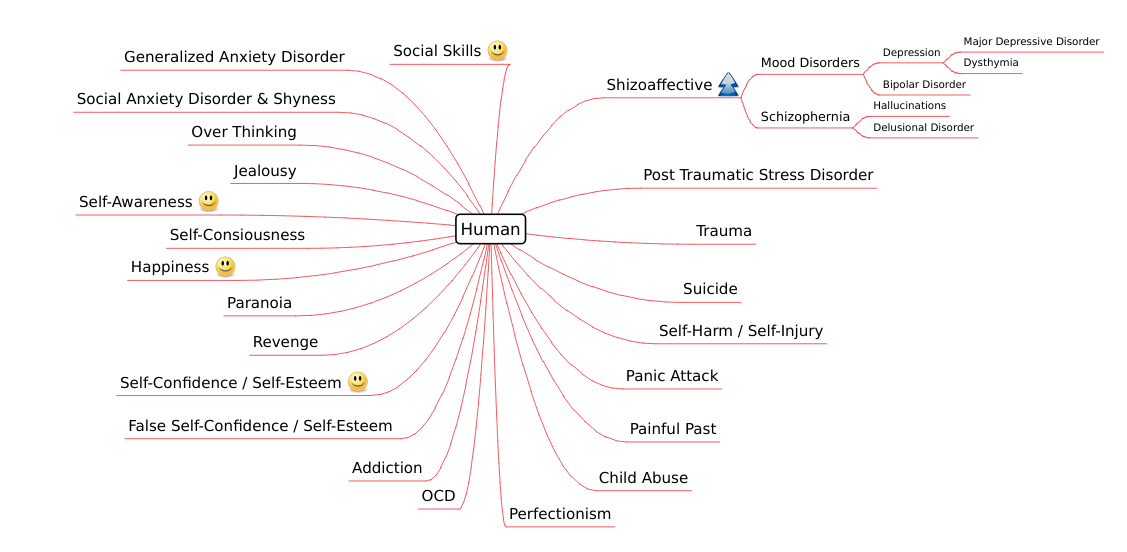
\includegraphics[width=\textwidth]{human.png}
\end{figure}

In case you also want to add to the list, consider the points below:
\begin{enumerate}
    \item The author should have a PhD degree in related topic.
    \item The author should be an expert in that field.
    \item The author's methods must be applicable.
\end{enumerate}

\newpage
% \tableofcontents
% \newpage

\section{Social Skills}
\begin{itemize}
    \item The Social Skills Guide Book
    \item How to Win Friends and Influence People
    \item Conversationally Speaking
    \item How to Speak, How to Listen
\end{itemize}
\begin{additional}
    \item Improve your Social Skills
\end{additional}

\section{Generalized Anxiety Disorder}
\begin{itemize}
    \item Generalized Anxiety Disorder Work Book: A Comprehensive CBT Guide
    \item Rewire your Anxious Brain
\end{itemize}
\begin{additional}
    \item Cognitive Behavioral Anxiety Disorder Treatment for Generalized
    \item The Anxiety and Worry Workbook: The Cognitive Behavioural Solution
    \item Generalized Anxiety Disorder: Advances in Research and Practice
\end{additional}

\section{Social Anxiety Disorder \& Shyness}
\begin{itemize}
    \item The Shyness \& Social Anxiety Workbook
    \item Overcoming Social Anxiety \& Shyness
\end{itemize}

\section{Overthinking}
\begin{itemize}
    \item The Worry Trick
    \item Soundtracks: The Surprising Solution to Overthinking
\end{itemize}

\section{Self-confidence / Self-esteem}
\begin{itemize}
    \item The Confidence Gap
    \item The Self-confidence Workbook
\end{itemize}
\begin{additional}
    \item Self-esteem: A Proven Program of Cognitive Technique
    \item How to be yourself
\end{additional}


\end{document}
